\section{Theoretical Analysis of Co-Training}
\label{sec: theoretical insight}

% In this section, we introduce two intrinsic factors of sim-and-real co-training - co-training ratio and observation representations.
% This section sets a theoretical perspective for us to understand how co-training ratio affects the model.
Generative robot policies use generative modeling architectures, such as diffusion/flow models, and autoregressive transformers, as parameterizations of the mapping from observation to action.
Given their popularity and adoption in industry, our analysis throughout this paper focuses on the most popular policy form --- diffusion/flow matching policy~\cite{chi2025diffusion}. 
In the following, we use ``diffusion'' as an umbrella term for both diffusion and flow matching~\cite{liu2022flow} models, as they are equivalent under our analysis~\cite{gao2025diffusion}.
% We start by introducing a general unconditional diffusion model (Sec.~\ref{sec:2.1}); then, we analyze co-training with unconditional generation (Sec.~\ref{sec:merge}); further, we extend our analysis to sim-and-real co-training (Sec.~\ref{sec: condition representation}).
We start with illustrating why structured representation alignment matters in co-training with diffusion policy (Sec.~\ref{sec: condition representation}); then, we provide an analysis of the importance reweighting effect (Sec.~\ref{sec: balanced mixing ratio}).

% \subsection{Co-Training with Diffusion Policy}
\subsection{Structured Representation Alignment}
\label{sec: condition representation}
Training diffusion policy corresponds to jointly learning a feature encoder $f_\phi:\mathcal{O}\rightarrow\mathcal{Z}$ to project observations into a latent space, and a policy model $\pi_\theta:\mathcal{Z}\rightarrow\mathcal{A}$ that maps the learned representations to the action space.
Formally, given limited robotic dataset $\mathcal{D}_T=\{(o_i, a_i)\}_{i=1}^N$ in the target domain, and abundant dataset $\mathcal{D}_S=\{(o_j, a_j)\}_{j=1}^M$ from a source domain ($M \gg N$), we train a diffusion policy model ~\cite{chi2025diffusion} with mixing ratio $w$. 
This gives us the learning objective as:
\begin{equation}
    \mathcal{L}_{w}(t; \phi,\theta) := w \cdot \mathcal{L}_{\mathcal{D}_T} + (1-w) \cdot \mathcal{L}_{\mathcal{D}_S}
\label{eq: cotrain dp}
\end{equation}
where $\mathcal{L}_{\mathcal{D}} = \mathbb{E}_{(o_i, a_i) \sim \mathcal{D}, \epsilon \in \mathcal{N}(\mathbf{0}, \mathbf{I}_d)} [||\epsilon - \epsilon_\theta(a^t, t, o)||_2^2]~$.
We can prove that there exists an analytical optimal solution.
In this paper, we adopt the score parameterization (proof provided in Appendix~\ref {appdx: demonstration}):
\begin{equation}
    s_w^*(a^t,t,o)=\hat{w}_t\cdot s_t^*(a^t,t,o) + \hat{w}_s\cdot s_s^*(a^t,t,o)~
\end{equation}
where 
\begin{equation}
\begin{aligned}
    \hat{w}_t
    &= \frac{w\cdot p_t(a^t,f_\phi(o))}
    {w\cdot p_t(a^t,f_\phi(o)) + (1-w)\cdot p_s(a^t,f_\phi(o))} \\
    p_k(a^t, z)
    &= \frac{1}{|\mathcal{D}_k|}
    \sum_{i\sim \mathcal{D}_k}
    p(a^t|a_i^0)\cdot K(z, z_i),
    \quad k\in\{t,s\}.
\end{aligned}
\label{eq: conditional w}
\end{equation}

Here $K(\cdot, \cdot)$ is a kernel measuring how closely the current observation matches the observations in the dataset. So the behavior of the empirical optimal score function depends heavily on the learned observation representations $z = f_\phi(o)$. Based on the degree of representation alignment between the source and the target domain induced by $f_\phi$, we hypothesize three different scenarios in co-training: 1) \textbf{Disjoint:} observation representations of source and target domains are located in totally different clusters. During inference in the target domain, with $p_s(a^t,z)\approx 0$, the dynamic weight $\hat{w}_t$ stays near $1$. So the policy ignores data from the source domain, thus no \textit{positive transfer} from source to target will occur. 2) \textbf{Structured aligned:} the policy learns task-relevant, domain-invariant representations while retaining sufficient domain-specific information, such that observation representations of source and target domains are close but not collapsed. In this case, the action prediction will be effectively guided by neighbors in the source domain but dominated by data from the target domain. This informs our definition of structured representation alignment at the beginning. 3) \textbf{Overlapping:} Although the observation representations of the source and target domains are fully aligned, the corresponding actions differ due to domain gaps. As a result, the policy prediction is unaware of the actual environment and instead exhibits a bimodal distribution over source and target actions, leading to \textit{negative transfer}.

% \begin{itemize}[leftmargin=*]
%     \item \textbf{Disjoint:} observation representations of source and target domains are located in totally different clusters. 
%     During inference in the target domain, with $p_s(x^t,z)\approx 0$, the dynamic weight $\hat{w}_t$ stays near $1$. 
%     So the policy ignores data from the source domain, thus no \textit{positive transfer} from source to target will occur.
%     \item \textbf{Structured aligned:} the policy learns task-relevant, domain-invariant representations while retaining sufficient domain-specific information, such that observation representations of source and target domains are close but not collapsed.
%     In this case, the action prediction will be effectively guided by simulation neighbors but dominated by data from the target domain.
%     \item \textbf{Overlapping:} Although the observation representations of the source and target domains are fully aligned, the corresponding actions differ due to domain gaps. As a result, the policy prediction is unaware of the actual environment and instead exhibits a bimodal distribution over source and target actions, leading to \textit{negative transfer}.
% \end{itemize}

\subsection{Importance Reweighting Effect}
\label{sec: balanced mixing ratio}
% \todo{need to reframe this section}
Mixing ratio directly provides additional modulation in this transfer process. Given any specific observation $o$, Eq.~\eqref{eq: conditional w} will degrade to:
\begin{equation}
    \hat{w}_t := \frac{w p_t(a^t)}{w p_t(a^t) + (1-w) p_s(a^t)}
\label{eq: unconditional w}
\end{equation}
where $p_t(a^t) = \frac{1}{N} \sum_{i:o_i=o}^{N} p(a^t|a^0=a_i), p_s(a^t) = \frac{1}{M} \sum_{j:o_j=o}^{M} p(a^t|a^0=a_j)$. 
% (The detailed proof and derivation is provided in the \textbf{Appendix xxx}).
% From a high-level perspective, co-training can be viewed as merging two score fields with time-dependent weights specified by $w$.
At a large $t$ during inference, as data are greatly perturbed by noise, $p_t(a^t)\approx p_s(a^t)$, the model will approximate a global average between two domains;
at a smaller $t$, $p(a^t)$ will be concentrated on one domain with the existence of domain gaps, so the model prediction will converge to one specific domain with $\hat{w_t}\approx 1$. 
At any timestep $t$, as $a^t$ are usually distributed as Gaussians around the training sample, for each data point we define: $r_k(a^t,t) := \frac{||a^t - \alpha_t a_k||}{\sigma_t \sqrt{d}}$.
We can have a closer look at the merged score function with further simplifications:
\begin{equation}
\begin{aligned}
    s_w^*(a^t,t) = &\sum_{i_t}^N g_{i_t}s^*_{i_t} + \sum_{i_s}^Mg_{i_s}s^*_{i_s}
    \\
    g_{i_k}=Softmax(\ln(w_k) &- r_k^2(a^t,t)* d/2), \quad k\in\{t,s\} \\
    w_t = w/N&, w_s = (1-w)/M ~
\end{aligned}
\label{eq: softmax}
\end{equation}
where $s_i^*$ is the optimal score towards each action data (derivation provided in Appendix~\ref{appdx: derivation}).
It reshapes the action sampling distribution to learn by reweighting the score functions in two domains during training as shown below.
\begin{figure}[htbp]
    \centering
    \captionsetup{font={small}}
    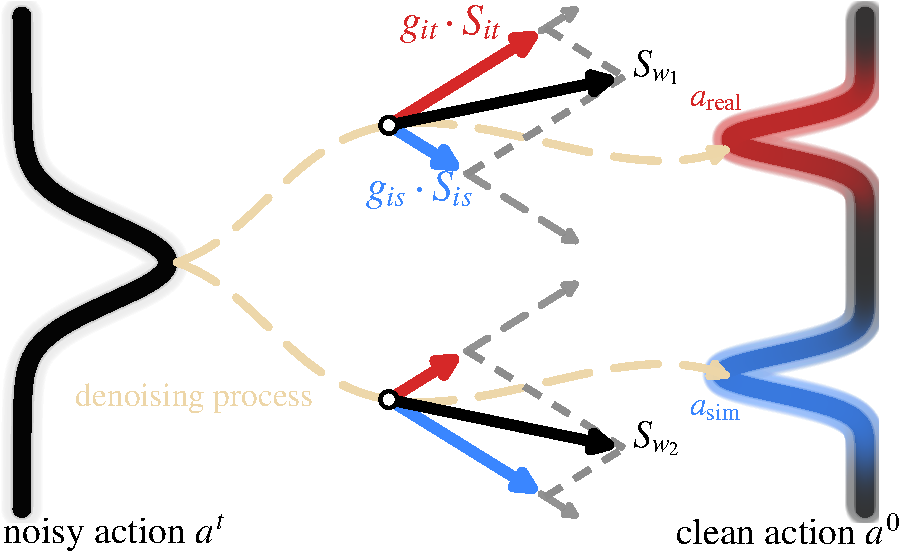
\includegraphics[width=0.9\linewidth]{asset/teaser_small.pdf}
    % \vspace{-10pt}
    \caption{Importance reweighting reshapes the learned action distribution via reweighting score functions during training time.}
    \label{fig: reweight}
    \vspace{-20pt}
\end{figure}

% By further simplification, we can have a closer look at the merged score function $s_w^*(a^t,t)= \frac{1}{\sigma_t^2} [\alpha_t \mathbf{C} - a^t]$ (derivation provided in Appendix~\ref{appdx: derivation}):
% \begin{equation}
% \begin{aligned}
%     \mathbf{C}(a^t,t) &= \sum_{k=1}^{N+M} Softmax(\ln(w_k) - r_k^2(a^t,t)* d/2) \cdot a_k \\
%         w_k &= \left\{\begin{aligned}
%              \frac{w}{N} && \text{for $k={1,\cdots, N}$} \\ 
%              \frac{1-w}{M} && \text{for $k=\{N+1, \cdots, N+M\}$}~
%         \end{aligned}\right.
% \end{aligned}
% \label{eq: softmax}
% \end{equation}

\begin{figure*}[tbp]
\centering
    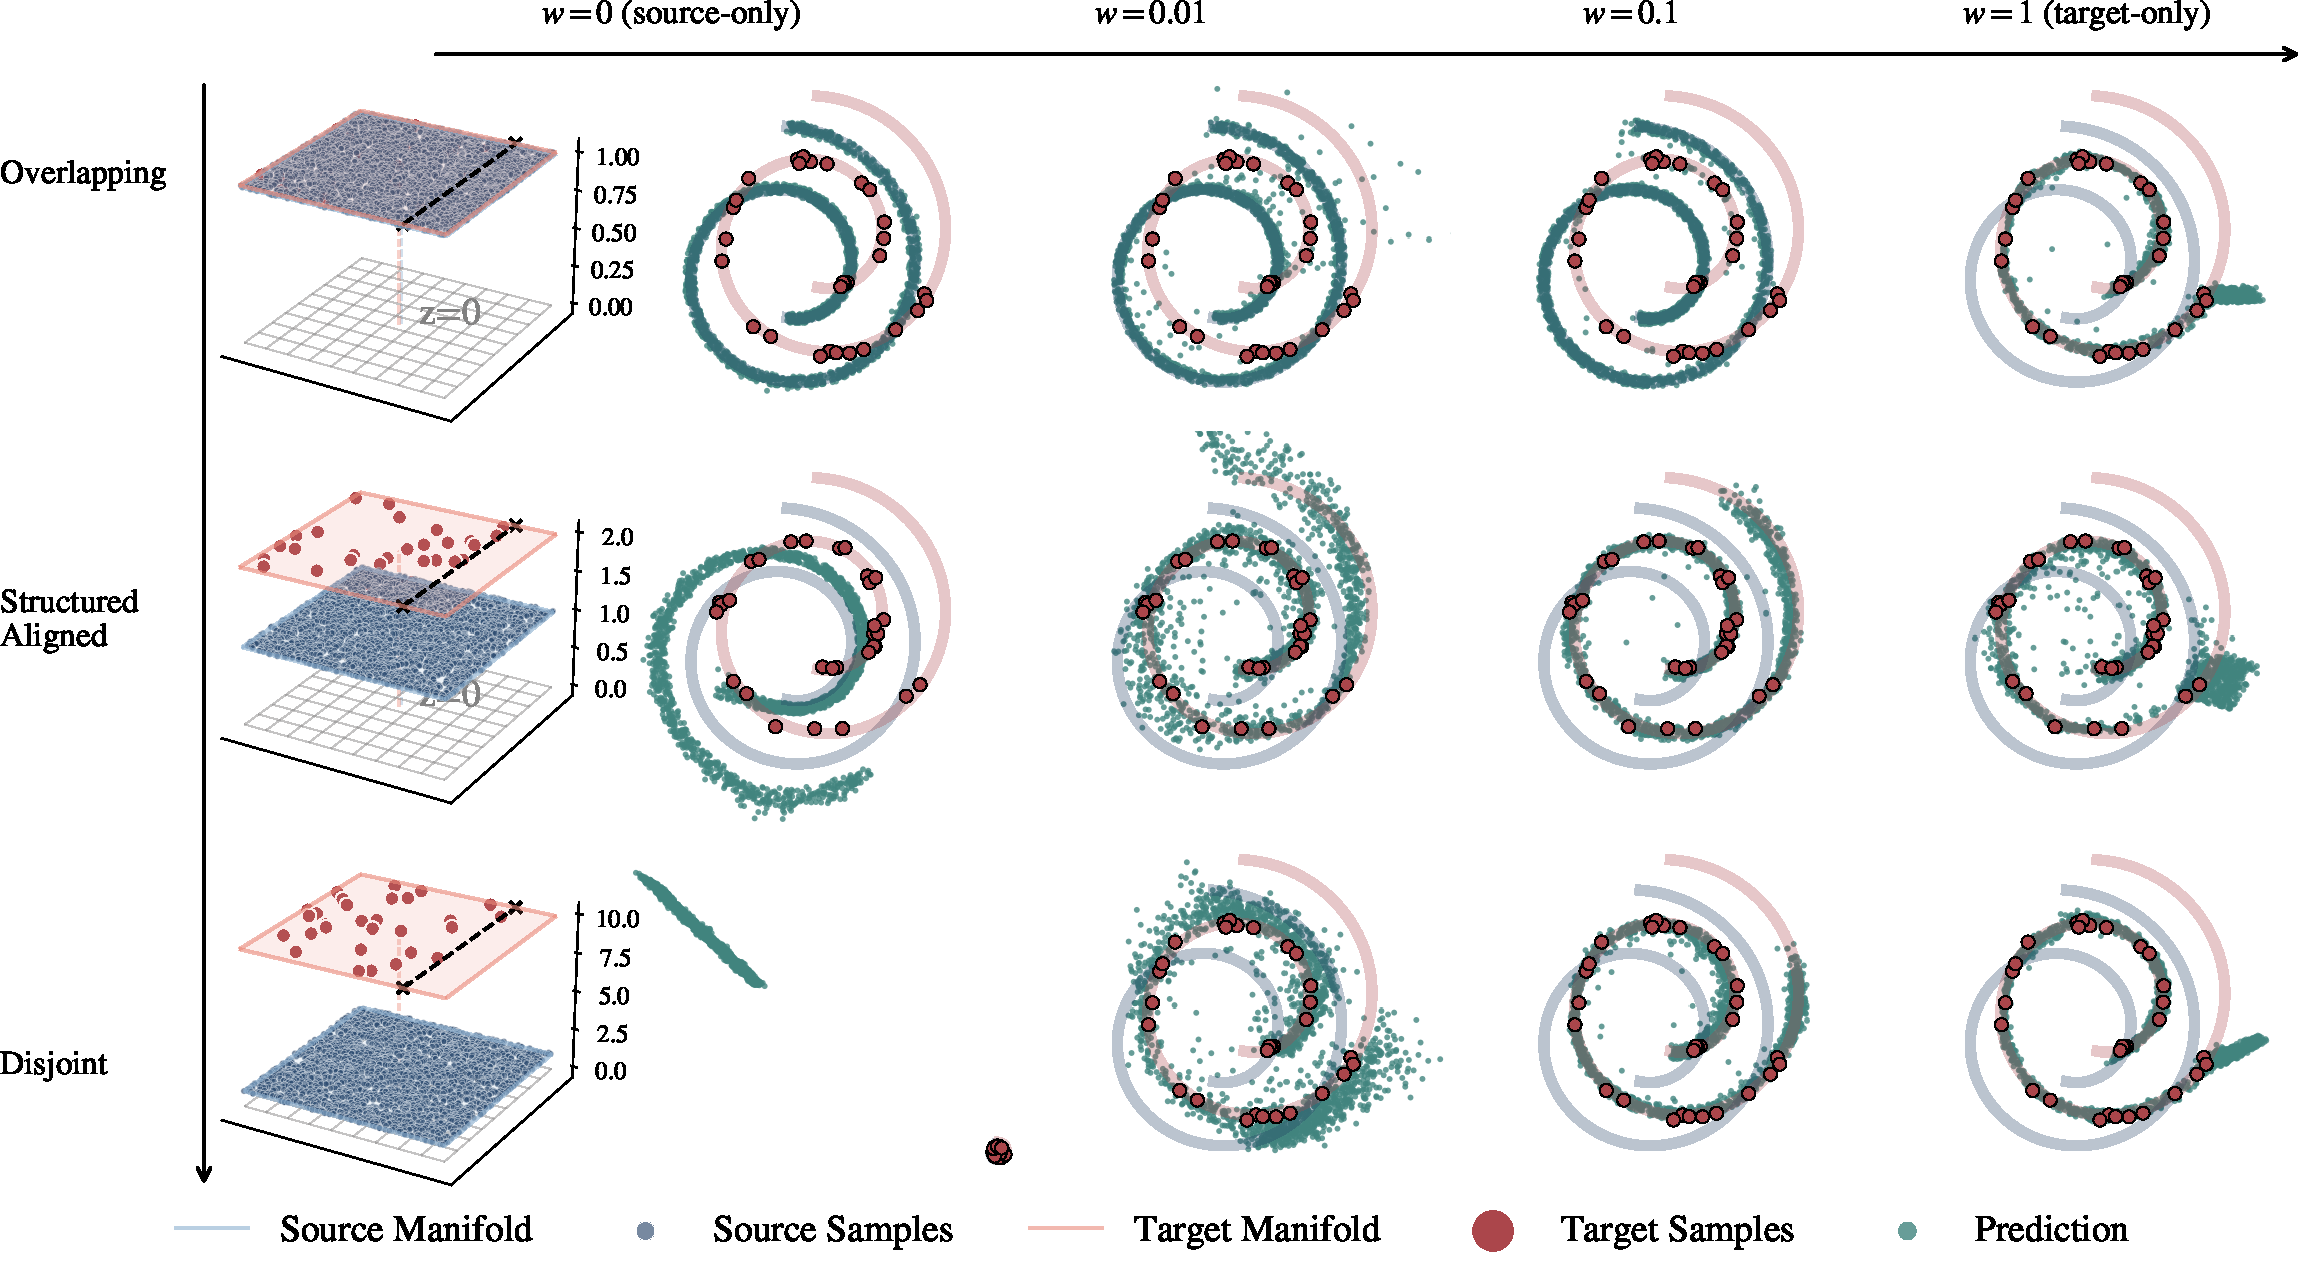
\includegraphics[width=0.93\linewidth]{asset/toy_example.pdf}
    \caption{\textbf{Visualization of controlled toy example.} We co-train $\sim$30 and $\sim$3000 samples from target and source domain.
    Vertically in each column, the differences of prediction samples showcase the impact of representation alignment; horizontally in each row, the differences showcase the shift of importance reweighting effect controlled by mixing ratio $w$.}
    \label{fig:toy-example}
\end{figure*}
% Following ~\citet{wei2025empirical}, we define \textit{natural co-training ratio} $w_n:=\frac{N}{N+M}$, where $w_k$ between domains are the same, equaling to directly concatenating datasets in practice.
% When $w > w_n$, compared to the samples in the source dataset, samples in the target dataset are assigned higher weights. 
In a special case, we can further have the following relation of the relative weight ratio:
\begin{equation}
\begin{aligned}
    \frac{g_{i_t}}{g_{i_s}} \propto \mathcal{F}(\frac{w}{1-w}, \frac{M}{N}, |a_{i_t}-a_{i_s}|)
\end{aligned}
\end{equation}
% It can be seen that the supervision region specified by $\sigma_t\sqrt{d}$ for target samples becomes larger.
% So $w$ is changing the importance across domains but has no effect within each domain.
The amplitude of this modulation is influenced by both $w$, the dataset size and domain gaps.
A detailed characterization about this property is provided in Appendix~\ref {appdx: estimation}.
% Therefore, we define \textit{balanced mixing ratio} as a range where the samples in the source and target domains are assigned with comparable weights, but Eq.~\ref{eq: softmax} is mainly affected by samples in the target domain.
% An estimation of the balanced mixing ratio in this case on sim-and-real co-training is provided in Appendix~\ref {appdx: estimation}.
% Our key finding is that:

Based on the analysis above, we can summarize as follows:
\uline{{The effectiveness of} co-training with diffusion policy is mainly decided by two intrinsic effects:
(1) structured representation alignment; (2) the importance reweighting effect.}
With the above theoretical analysis, we are now ready to find empirical evidence that supports our insight.
